%iffalse
\let\negmedspace\undefined
\let\negthickspace\undefined
\documentclass[journal,12pt,twocolumn]{IEEEtran}
\usepackage{cite}
\usepackage{amsmath,amssymb,amsfonts,amsthm}
\usepackage{algorithmic}
\usepackage{graphicx}
\usepackage{textcomp}
\usepackage{xcolor}
\usepackage{txfonts}
\usepackage{listings}
\usepackage{enumitem}
\usepackage{mathtools}
\usepackage{gensymb}
\usepackage{comment}
\usepackage[breaklinks=true]{hyperref}
\usepackage{tkz-euclide} 
\usepackage{listings}
\usepackage{gvv}                                        
\def\inputGnumericTable{}                                 
\usepackage[latin1]{inputenc}                                
\usepackage{color}                                            
\usepackage{array}                                            
\usepackage{longtable}                                       
\usepackage{calc}                                             
\usepackage{multirow}                                         
\usepackage{hhline}                                           
\usepackage{ifthen}                                           
\usepackage{lscape}

\newtheorem{theorem}{Theorem}[section]
\newtheorem{problem}{Problem}
\newtheorem{proposition}{Proposition}[section]
\newtheorem{lemma}{Lemma}[section]
\newtheorem{corollary}[theorem]{Corollary}
\newtheorem{example}{Example}[section]
\newtheorem{definition}[problem]{Definition}
\newcommand{\BEQA}{\begin{eqnarray}}
\newcommand{\EEQA}{\end{eqnarray}}
\newcommand{\define}{\stackrel{\triangle}{=}}
\theoremstyle{remark}
\newtheorem{rem}{Remark}
\usepackage{float}
\begin{document}

\bibliographystyle{IEEEtran}
\vspace{3cm}

\title{Filter Design}
\author{EE23BTECH11017 - Eachempati Mihir Divyansh$^{*}$% <-this % stops a space
}
\maketitle
\newpage
\bigskip

\renewcommand{\thefigure}{\theenumi}
\renewcommand{\thetable}{\theenumi}

    \section{Introduction}
    We must design an IIR and FIR filter with a given filter number. This is a bandpass filter whose specifications are shown below.
    \section{Filter Specifications}
    The sampling rate for the filter has been specified as $F_s =  48$ kHz.	If the un-normalized discrete-time (natural) frequency is F, the corresponding normalized digital filter (angular) frequency is given by $\omega = 2\pi\brak{\frac{F}{F_s}}$.
    \subsection{Digital Filter}
    \begin{enumerate}
        \item \textit {Passband }: \\\{4 + 0.6\brak{j}\} kHz to \{4 + 0.6\brak{j+2}\} kHz, where 
        \begin{align}
            j = \brak{r - 11000} \mod \sigma
        \end{align}
        where $\sigma$ is the sum of the digits of my roll number and $r$ is the roll number.
        \begin{align}
            r &= 11017 \\
            \sigma &= 10 \\
            j &= 7
        \end{align}
        So, the un-normalized, discrete-time passband frequencies are 
        \begin{align}
            F_{p_1} = 8.2\text{ kHz}\\
            F_{p_2} = 9.4\text{ kHz}
        \end{align}
        The corresponding normalized digital frequencies are: 
        \begin{align}
            \omega_{p_1} = 2\pi \frac{F_{p_1}}{F_s} = 0.34 \pi\\
            \omega_{p_2} = 2\pi \frac{F_{p_2}}{F_s} = 0.39 \pi \\
            \omega_{c} = \dfrac{\omega_{p_1}+\omega_{p_2}}{2}
            \end{align}
            Where $\omega_c$ is the center frequency.

        \item \textit {Tolerance: }The deviations in the passband and stopband ($\delta_p$ and $\delta_s$) are called the tolerances of a filter. Assuming that they are equal, let 
        \begin{align}
            \delta_p = \delta_s = 0.15
        \end{align}
        \item \textit {Stopband}: The transition band on either side of the passband is given to be \begin{align}
            \Delta F = 0.3 \text{ kHz}
        \end{align}
        Therefore, 
        \begin{align}
            F_{s_1} = F_{p_1} - \Delta F = 7.9 \text{ kHz}\\
            F_{s_2} = F_{p_2} + \Delta F = 9.7 \text{ kHz}
        \end{align}
        and the corresponding normalized digital frequencies are: 
        \begin{align}
            \omega_{s_1} = 0.33 \pi\\
            \omega_{s_2} = 0.40 \pi 
            \end{align}
        \end{enumerate}
        \subsection{Analog Filter} \label{filt_param}
        The analog filter frequency is related to the digital frequency by 
        \begin{align}
            &\Omega = \tan \frac{\omega}{2} \\
            \implies &\Omega_{p_1} = 0.59,\; \Omega_{p_2} = 0.70,\\ \implies &\Omega_{s_1} = 0.57 ,\; \Omega_{s_2} = 0.74
        \end{align}
    \section{The IIR Filter Design}
    For the design of our bandpass IIR filter, we require a stopband with a monotonic characteristic and an equiripple passband. Consequently, the Chebyshev approximation is employed.
    \subsection{The Analog Filter}
\begin{enumerate}

\item\textit{Low Pass Filter Specifications:}  Let $H_{a, BP}\brak{j\Omega}$ be the desired analog bandpass filter,  with the specifications provided in \ref{filt_param}, and $H_{a, LP}\brak{j\Omega_L}$ be the equivalent low pass filter. Define 
\begin{align}
    \Omega_0 = \sqrt{\omega_{p_1}\omega_{p_2}} = 0.64 \\
    B = \omega_{p_2} - \omega_{p_1} = 0.11
\end{align}
Then, 
\begin{equation}
\Omega_L = \frac{\Omega^2 - \Omega_0^2}{B\Omega} \label{eq:freq_transform}
\end{equation}
Substituting $\Omega_{s_1}$ and $\Omega_{s_2}$ in \eqref{eq:freq_transform} we obtain the stopband edges of lowpass filter 
\begin{align}
    \Omega_{Ls1} &= \frac{\Omega_{s_1}^2 - \Omega_0^2}{B\Omega_{s_1}} = -1.50\\
    \Omega_{Ls2} &= \frac{\Omega_{s_2}^2 - \Omega_0^2}{B\Omega_{s_2}} = 1.56
\end{align}
We choose the minimum of these two stopband edges
\begin{align}
    \Omega_{Ls} = \mbox{min}\brak{\abs {\Omega_{Ls_1}},\abs \Omega_{Ls_2}} = 1.50
\end{align}
\item \textit{The Low Pass Chebyschev Filter Parameters:} The magnitude of an $n$th order Chebyschev low-pass filter transfer function  is given by: 
\begin{align}
     H_{a,LP}\brak{j\Omega_L} = \dfrac{1}{\sqrt{1 + \varepsilon^2T_N^2\brak{\Omega_L/\Omega_{Lp}}}} \label{eq:mag_freq_response}
\end{align}
where $$\varepsilon = \sqrt{10^{\delta_p/10}-1}$$ is the ripple factor, $\Omega_{Lp}$ is the cutoff frequency and $$T_n \brak{x}= \cosh{\brak{N \cosh ^{-1} x}}$$ is a Chebyshev polynomial of the $n$th order. 
The recurrence relation for the polynomials is as follows
\begin{align}
    T_{N+2} &= 2xT_{N+1} - T_{N}  \label{eq:cheby_poly_relation}
\end{align}
The filter parameters have the following constraints
\begin{align}
\label{lpdesign}
\frac{\sqrt{D_2}}{c_N\brak{\Omega_{Ls}}} \leq \varepsilon \leq \sqrt{D_1}  \\
N \geq \left\lceil \frac{\cosh^{-1}\sqrt{\dfrac{D_2}{D_1}}}{\cosh^{-1}\Omega_{Ls}} \right\rceil
\end{align}
where $D_1 = \dfrac{1}{(1 - \delta)^2}-1$ and $D_2 = \dfrac{1}{\delta^2} - 1$ and $\left \lceil . \right \rceil$ is known as the ceiling operator. \\ \\
After the necessary substitutions, we get N $\geq$ 4 and 0.278 $\leq \varepsilon \leq$ 0.61.
Plotting the magnitude of the transfer function vs $\varepsilon$, we get
\renewcommand\thefigure{\thesection-\arabic{figure}} 
\begin{figure}[H]
    \centering
    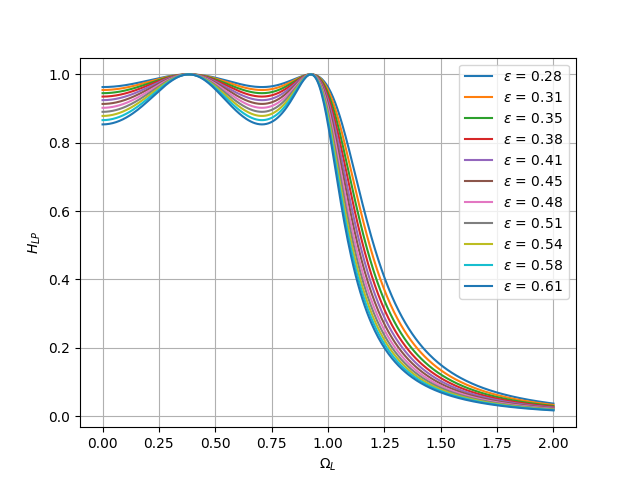
\includegraphics[width = \columnwidth]{figs/HvE.png}
    \label{fig:var_eps}
    \caption{Analog Low-Pass Frequency Response for $0.28 \leq \varepsilon \leq 0.61$}
\end{figure}
As the value of $\varepsilon$ increases, the roll-off becomes steeper. We choose $\varepsilon = 0.29$, as it perfectly transitions from the passband to the stopband.
\item \textit{The Low Pass Chebyschev Filter:} The next step in design is to find an expression for magnitude response in the $s$ domain. 

Using $s=j\Omega$ or in this case $s_{L}=j\Omega_{L}$ we obtain:
\begin{align}
    \abs{ H_{a,LP}(j\Omega_L)}^2 = \dfrac{1}{1 + \epsilon^2T_N^2(\frac{s_L}{j})}
\end{align}
To find poles equate the denominator to zero:
\begin{align}
    {1 + \epsilon^2T_N^2\brak{\dfrac{s_L}{j}}} &=0 \label{eq:pole_ques}
\end{align}
where 
\begin{align}
    T_N(x) &= \cos{\brak{N\cos^{-1}{\brak{x}}}},  \;\abs{x} < 1  \\
    T_N(x) &= \cosh{\brak{N\cosh^{-1}{\brak{x}}}},  \;\abs{x}\geq 1
\end{align}
On solving \eqref{eq:pole_ques} we obtain poles :
\begin{align}
    s_{k} &= -\Omega_{Lp} \sin\brak{A_k}\sinh\brak{B_k} - j\Omega_{Lp}\cos\brak{A_k}\cosh\brak{B_k}
\end{align}
where $k$ is the index of the pole and \\
\begin{align}
    A_k &= \brak{2k+1}\dfrac{\pi}{2N}\\
    B_k &= \dfrac{1}{N} \sinh^{-1}{\brak{\dfrac{1}{\epsilon}}}
\end{align}
The $s_k$ values, calculated and plotted by the following Python code are as follows: 
\begin{lstlisting}
https://github.com/Mihir-Divyansh/EE1205/blob/main/Filter_Design/codes/sk.py
\end{lstlisting}
\renewcommand\thetable{\thesection-\arabic{table}} 
\begin{table}[H]
    \centering
    \resizebox{0.6\columnwidth}{!}{%
    \begin{tabular}{|c|c|c|}
    \hline
    \textbf{Pole} & \textbf{Value} \\ \hline
    $s_1$ &0.460 + 0.428\j \\ \hline
    $s_2$ &0.460 - 0.428\j \\ \hline
    $s_3$ &0.191 - 1.032\j  \\ \hline
    $s_4$ &0.191 + 1.032\j\\ \hline
    $s_5$ &-0.191 - 1.032\j\\ \hline
    $s_6$ &-0.460 - 0.428\j\\ \hline
    $s_7$ &-0.460 + 0.428\j  \\ \hline
    $s_8$ &-0.191 + 1.032\j \\ \hline
    \end{tabular}%
    }
    \caption{Values of $s_k$}
    \label{tab: values of poles sk}
    \end{table}
The poles in the left half of the plane i.e., with -ve real part are taken in the filter design as we intend to design a stable system.

\begin{figure}[H]
    \centering
    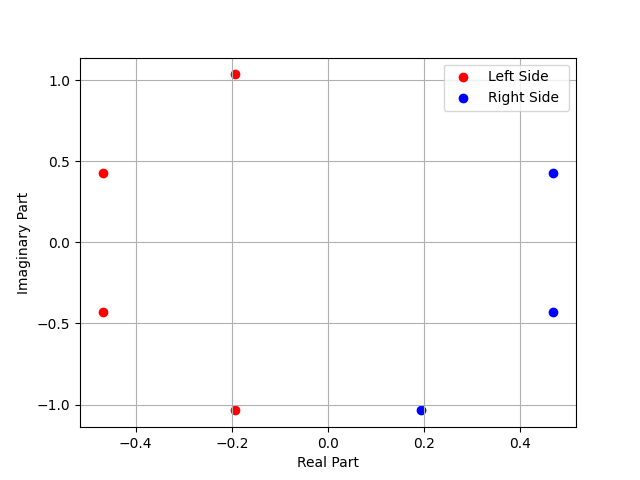
\includegraphics[width = \columnwidth]{figs/sk_pole_zero.png}
    \caption{Pole-Zero Plot}
    \label{fig:pzplot}
\end{figure}
\begin{align}
    H_{a,LP}(s_L) &= \frac{G_{LP}}{\brak{s_L-s_5}\brak{s_L-s_6}\brak{s_L-s_7}\brak{s_L-s_8}} \label{eqn: magres}
\end{align}
where $G_{LP}$ is the gain of the Low pass filter. Refer to \tabref{tab: values of poles sk} for $s_k$ values.\\

We know that from \eqref{eq:mag_freq_response}:-
\begin{align}
    \abs{ H_{a,LP}(s_L)} &= \frac{1}{\sqrt{1+\epsilon^2}} \text{at} \hspace{5pt} \Omega_{L}=1 \implies s_{L} = j \label{eq:Gain_eq_LP} 
\end{align}
Substituting values from \eqref{eq:Gain_eq_LP} in \eqref{eqn: magres} we get $G_{LP}=0.4166$ \\

\begin{footnotesize}
\begin{align}
    H_{a,LP}(s_L) = \frac{0.42}{s_{L}^4 + 1.30s_{L}^3 +1.85s_{L}^2 + 1.17s_{L} +0.43}\label{eq:design}
\end{align}
\end{footnotesize}
\begin{figure}
    \centering
    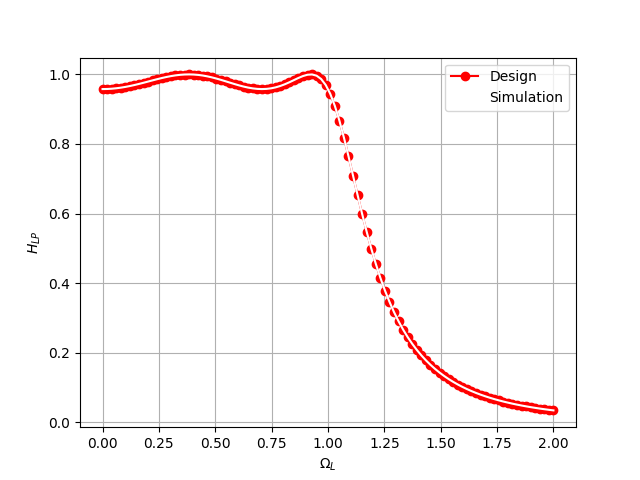
\includegraphics[width = \columnwidth]{figs/Design vs Simulation.png}
    \caption{Design v/s Simulation for the filter}
    \label{fig:desVsim}
\end{figure}

\item \textit{The Band Pass Chebyschev Filter:} 
After verifying the design with the required specifications the next step is to jump to the required type of filter using frequency transformation. 
\begin{align}
    s_L &= \frac{s^2 + \Omega_0^2}{Bs} \\
    H_{a,BP}(s) &= G_{BP}H_{a,LP}(s_L)\vert_{s_L = \frac{s^2 + \Omega_0^2}{Bs}}
\end{align}
As there is one-to-one correspondence between the filters so $\Omega=\omega_{p_1}$ should correspond to $\Omega_{Lp}$
\begin{align}
    &s = j\omega_{p_1}\\
    &s_{L} = \frac{(j\omega_{p_1})^2 + \Omega_0^2}{B(j\omega_{p_1})} \label{eq:res1} \\ 
    &\abs{H_{a,BP}(j\omega_{p_1})} = 1 \\
    &G_{BP}\abs{H_{a,LP}(s_L)} = 1 \label{eq:res2}
\end{align}
Substituting \eqref{eq:res1} in \eqref{eq:res2} we obtain Gain of required bass pass filter:
\begin{align}
    G_{BP} &= 1.04 
\end{align}
Thus the response in the \textit{s} domain 
\begin{tiny}
\begin{align}
    H_{a,BP}\brak{s} &= \dfrac{6.49\times 10^{-5}s^4}{s^8 + 0.14s^7 + 0.17s^6 + 0.18s^5 + 1.05s^4 + 0.75s^3 + 0.29s^2 + 0.01s + 0.03}  \label{eq:magnitude_bandpass_analog}
\end{align}
\end{tiny}
The expressions in the s-domain and gain factors have been computed using Python code.\\ \\ In Figure \ref{fig:anlg_resp}, we present the magnitude of \( H_{a, BP}(j\Omega) \) as a function of \( \Omega \) for both positive and negative frequencies. The pass-band and stop-band frequencies depicted in the figure exhibit close alignment with those determined analytically through the bilinear transformation. 
\begin{figure}[h]
    \centering
    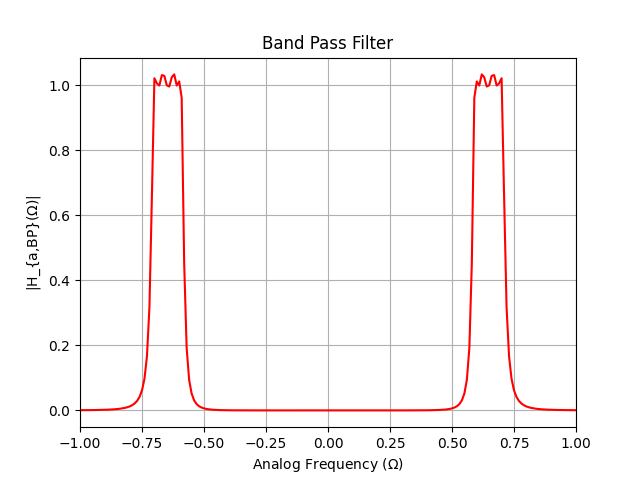
\includegraphics[width = \columnwidth]{figs/Band_Pass_Filter.png}
    \caption{Magnitude response of the Analog Band Pass Filter}
    \label{fig:anlg_resp}
\end{figure}
\end{enumerate}

\subsection{The Digital Filter}
From the bilinear transformation, we obtain the digital bandpass filter from the corresponding analog filter as
\begin{align}
    H_{d,BP}(z) = GH_{a,BP}(s)\big\vert_{s = \frac{1-z^{-1}}{1 + z^{-1}}}
\end{align}
Substituting $$s=\dfrac{1-z^{-1}}{1+z^{-1}}$$ in \eqref{eq:magnitude_bandpass_analog} and calculating expression using a python code we get :
\begin{tiny}
\begin{align}
    H_{d,BP}(z) &= \dfrac{G\brak{1 - 4z^{-2} + 6z^{-4} - 4z^{-6} + z^{-8}}}{3.62 - 6.95z^{-1} + 26.74z^{-2} - 60.15z^{-3} + 73.76z^{-4} - 49.57z^{-5} + 26.14z^{-6} - 7.62z^{-7} + 1.45z^{-8}}
\end{align}
\end{tiny}
where $G=6.49\times 10^{-5}$   \\ 
The plots for the filter magnitude by approximate calculation (using arrays) and symbolic math in Python are given below. The specifications for the filter are met.

\begin{figure}
    \centering
    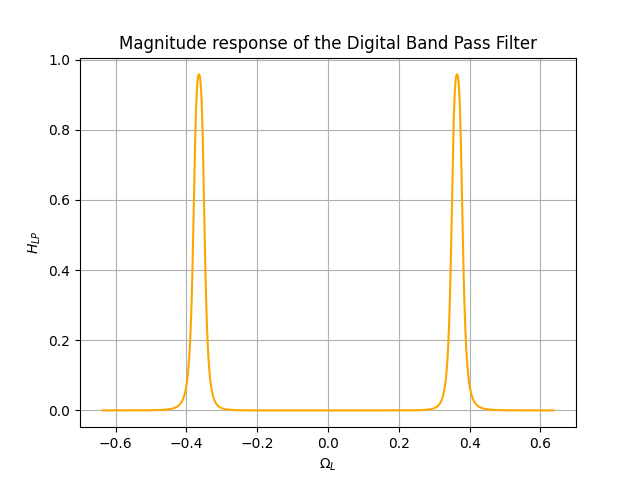
\includegraphics[width = \columnwidth]{figs/digital_bp.png}
    \caption{Approximation of the Filter}
    \label{fig:approx}
\end{figure}
\begin{figure}
    \centering
    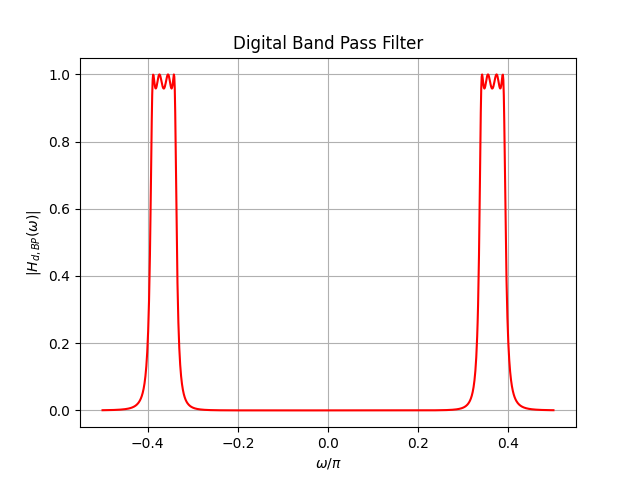
\includegraphics[width = \columnwidth]{figs/Digital_BPF.png}
    \caption{ Magnitude of the Digital Band Pass Filter}
    \label{fig:d,BP}
\end{figure}
\section{The FIR Filter}
We design the FIR filter by obtaining the (non-causal) lowpass equivalent using the Kaiser window and then converting it to a causal bandpass filter.
\subsection{The Equivalent Lowpass Filter}
The lowpass filter has a passband frequency $\omega_l$ and transition band $\Delta \omega = 2\pi \dfrac{\Delta F}{F_s} = 0.0125\pi$.
The stopband tolerance is $\delta_s = 0.15$.The cutoff-frequency is given by :
\begin{align}
    \omega_{Lp} &= \frac{B}{2} =  0.025\pi
\end{align}
The impulse response of the ideal Low Pass Filter is given by :
\begin{align}
    h\brak{n} = 
\begin{cases} 
    \frac{w_l}{\pi}, & \text{if } n = 0 \\
    \frac{\sin(w_l n)}{n\pi}, & \text{if } n \neq 0
\end{cases} \label{eq:h(n)_for_LPF}
\end{align}
From \eqref{eq:h(n)_for_LPF} we conclude that $h\brak{n}$ for an ideal Low Pass Filter is not causal and can neither be made causal by introducing a finite delay. And $h\brak{n}$ do not converge, so the system is unstable. Therefore we move on to windowing the impulse response.
\begin{figure}
    \centering
    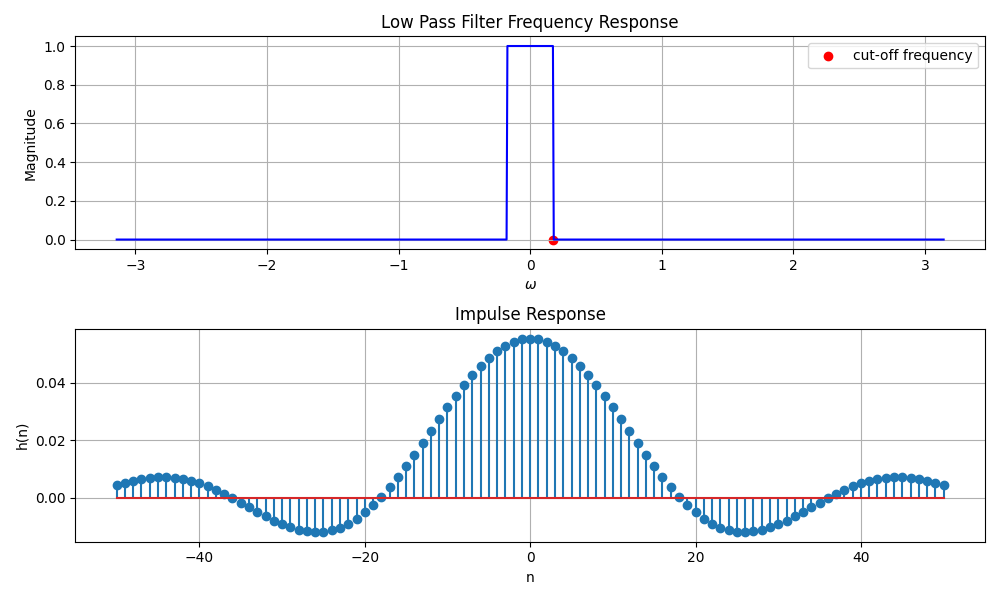
\includegraphics[width = \columnwidth]{figs/Impulse Response.png}
    \caption{Impulse Response of an Ideal Low Pass Filter}
    \label{fig:ideal_LPF}
\end{figure}
\subsection{The Kaiser Window}
The Kaiser window is defined as
\begin{align}
    w(n) =
    \begin{cases}
    \dfrac{I_0\left[ \beta N \sqrt{1 - \left(\frac{n}{N}\right)^2} \right]}{I_0(\beta N)},
\indent -N \leq n \leq N, \indent \beta > 0 \nonumber \\
 0, \hspace{2.5 cm} \mbox{otherwise}
 \end{cases}
\end{align}
where $I_0(x)$ is a modified Bessel Function of the first kind of zero order in $x$. $\beta$ and $N$ are the window-shaping factors.

\begin{enumerate}
\item  N is chosen according to
\begin{align}
    N \geq \dfrac{A-8}{4.57\Delta \omega},
\end{align}
where $A = -20\log_{10}\delta$.  Substituting the appropriate values from the design specifications, we obtain
$A = 16.4782$ and $N \geq 48$.


\item  $\beta$ is chosen according to
\begin{small}
    \begin{align}
    \beta N = \left\{ \begin{array}{ll} 0.11(A-8.7) & A > 50 \\
0.58(A-21)^{0.4}+ 0.08(A-21) & 21 \leq A \leq 50 \\
0 & A < 21\end{array} \right.
\end{align}
\end{small}


The window function is defined as :
\begin{align}
    w\brak{n} = 
\begin{cases} 
    1, & \text{for } -48\leq n \leq 48 \\
    0, & \text{otherwise } 
\end{cases} \label{eq:w(n)_for_Kaiser}
\end{align}
Therefore the desired impulse response is :
\begin{align}
    h_{lp} &= h_{n}w_{n}
\end{align}
\begin{align}
    h\brak{n} = 
\begin{cases} 
    \dfrac{\sin(w_l n)}{n\pi},  & \text{for } -48\leq n \leq 48 \\
    0 &\text{otherwise}
\end{cases} \label{eq:h(n)desired_for_LPF}
\end{align}
\end{enumerate}
\begin{figure}
    \centering
    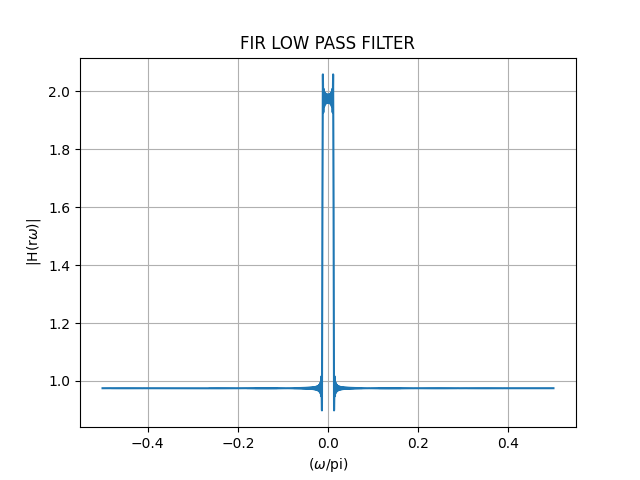
\includegraphics[width = \columnwidth]{figs/FIR_Lowpass_Filter.png}
    \caption{Magnitude Response of the FIR Low Pass Filter}
    \label{fig:fir_lpf}
\end{figure}
\subsection{The Equivalent Band Pass Filter}
A Band-Pass Filter (BPF) can be obtained by subtracting the magnitude response of a Low-Pass Filter (LPF) with cutoff frequency $\omega_{p_1}$ from another LPF magnitude response with cutoff frequency $\omega_{p_2}$.

\begin{align}
    h_{BP}\brak{n} = 
\begin{cases} 
    \dfrac{\sin(\omega_{p_2} n)}{n\pi} -\dfrac{\sin\brak{\omega_{p_1}n}}{n\pi},  & \text{for } n\neq 0\\\
    \dfrac{\omega_{p_2}-\omega_{p_1}}{\pi} &\text{for } n= 0
\end{cases} \label{eq:h(n)desired_for_LPF}
\end{align}
\begin{footnotesize}
    \begin{align}
     \dfrac{\sin(\omega_{p_2} n)}{n\pi} -\dfrac{\sin\brak{\omega_{p_1}n}}{n\pi} &= 2\cos{\brak{\frac{\omega_{p_2}n+\omega_{p_1}n}{2}}}\sin{\brak{\dfrac{\omega_{p_2}n-\omega_{p_1}n}{2}}}\\
            &= \dfrac{2\cos{\brak{0.37n\pi}}\sin{\brak{0.02n\pi}}}{n\pi}
\end{align}
\end{footnotesize}


Multiplying by window function we get :
\begin{align}
    h_{BP}\brak{n} = 
\begin{cases} 
   \frac{2\cos{\brak{0.37n\pi}}\sin{\brak{0.02n\pi}}}{n\pi},  & \text{for } \abs{n} \leq 48 \\
    0 &\text{otherwise}
\end{cases} \label{eq:h(n)desired_for_LPF}
\end{align}
\begin{figure}[t]
    \centering
    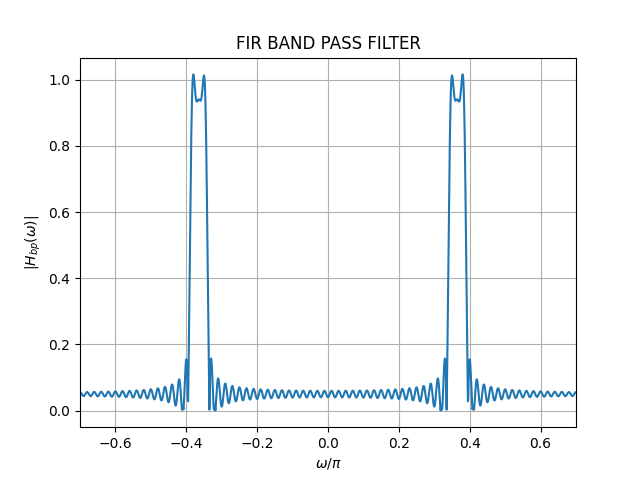
\includegraphics[width = \columnwidth]{figs/FIR_Bandpass_Filter.png}
    \caption{Magnitude Response of the FIR Band Pass Filter}
    \label{fig:fir_bpf}
\end{figure}
\end{document}
